\section{Experiments}
\label{sec:experiments}

\subsection{Setup}
Table~\ref{tab:setup} summarizes the layout, job model, planner parameters, and configurations. All configurations use $\eta=\eta'=16$~s, $\delta=10$~s, $\lambda=1.0$, and $v=1$~m/s; lift links use their configured 40~m length (40~s non-stop travel). The main comparison uses 100 jobs, 20 AGVs, seeds 1--10, and the strict track rule; the fleet sweep uses 4, 8, 12, 16, and 20 AGVs over the same job-generation settings. Every generated schedule is passed to an independent verifier that checks route endpoints, node and bidirectional-track separation, edge travel durations, dwell windows, and exactly-once job service; a run is accepted only when the verifier returns no violations.

\begin{table*}[t]
\centering
\small
\caption{Experimental setup (layout, job model, parameters, configurations).}
\label{tab:setup}
\resizebox{\textwidth}{!}{
\begin{tabular}{ll}
\toprule
Layout & 3 floors; 27 operational nodes (9 per floor); 38 edges; 4 lifts (40 m each); parking $\pi=$ 1A; 26 non-parking, non-lobby job stations \\
Jobs & pickup and delivery sampled uniformly from the 26 stations; $t_j\sim U[0,600]$ s; slack $s_j\sim U[30,200]$ s; $t'_j=t_j+d(p_j,p'_j)+\eta+\eta'+s_j$ \\
Fleet & 20 AGVs (\texttt{AGV-01}--\texttt{AGV-20}), fixed priorities $V_1$--$V_{20}$; fleet sweep: 4, 8, 12, 16, 20 AGVs \\
Parameters & $\eta=\eta'=16$~s; $\delta=10$~s; $\lambda=1.0$; $v=1$~m/s; lift travel 40~s \\
Main experiment & 100 jobs, 20 AGVs, seeds 1--10, strict track rule \\
Configurations & A: centralized paper-style (wait at parking only); B: centralized with lobbies; B2: centralized with lobbies and FCFS leg order; C: hybrid central + floor servers, lobbies, FCFS leg order \\
\bottomrule
\end{tabular}}
\end{table*}

\subsection{Main results: Gantt chart as main visual evidence}
Figure~\ref{fig:gantt-seed7} shows the A and C plans for seed 7 (100 jobs, 20 AGVs) on a shared time axis; rows are AGVs in priority order, colors are activities (moving on floor 1/2/3, lift trip, loading $\eta$, unloading $\eta'$), and hatched bars are waiting. Panel titles give data-derived totals. What to notice: under A the rows form a staircase of waiting that descends with priority. The annotation marks \GanttLongWaitAgvA{}: it waits \GanttLongWaitA~s before its first move under A but only \GanttSameAgvWaitC~s under C, while its service time is \GanttServiceSameAgv~s in both configurations — the same AGV's workload is unchanged, the waiting almost entirely disappears. Figure~\ref{fig:gantt-zoom} explains the hybrid: for \GanttZoomAgv{} (10 lift trips, floors 1--3), the route is cut into floor legs joined by lift trips, and the waiting between legs sits at lift lobbies rather than on floor nodes.

\begin{figure*}[t]
\centering
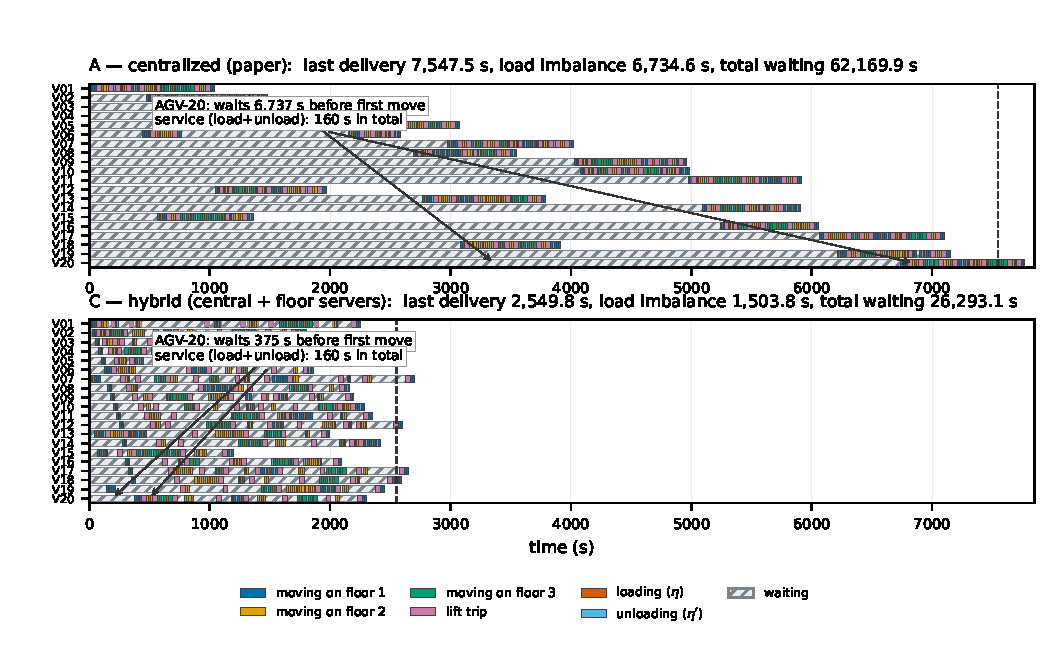
\includegraphics[width=\textwidth]{../figures/gantt_A_C_seed7.pdf}
\caption{How to read: each row is one AGV in priority order (V01 highest priority); colors are activities (moving on floor 1/2/3, lift trip, loading $\eta$, unloading $\eta'$); hatched bars are waiting. Panels show the seed-7 job set under A (top) and C (bottom) on a shared time axis; dashed vertical lines mark each panel's last delivery (the bars continue to the final return to parking). Under A the rows form a staircase of waiting that descends with priority. The annotation marks \GanttLongWaitAgvA{}: it waits \GanttLongWaitA~s before its first move under A but only \GanttSameAgvWaitC~s under C, while its service time is \GanttServiceSameAgv~s in both configurations. Panel titles give data-derived totals: last delivery \GanttPanelALastDelivery{} versus \GanttPanelCLastDelivery~s, load imbalance \GanttPanelAImbalance{} versus \GanttPanelCImbalance~s, total waiting \GanttPanelAWaitTotal{} versus \GanttPanelCWaitTotal~s.}
\label{fig:gantt-seed7}
\end{figure*}

\begin{figure}[t]
\centering
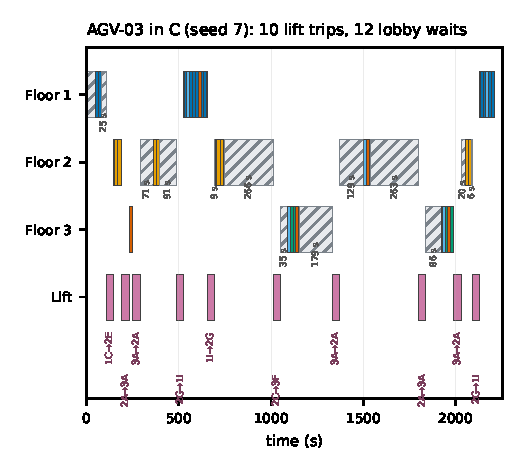
\includegraphics[width=\columnwidth]{../figures/gantt_zoom_seed7_agv-03.pdf}
\caption{How the hybrid builds one route, shown for \GanttZoomAgv{} on the same seed. Rows are the three floors and the lifts; the AGV's route is cut into floor legs joined by \GanttZoomLiftTrips{} lift trips (labelled with their lobby-to-lobby nodes). Hatched bars at lift-entry lobbies are lobby waits: \GanttZoomLobbyWaits{} waits totalling \GanttZoomLobbyWaitTotal~s. Between floor legs the AGV waits at lift lobbies rather than holding a floor node.}
\label{fig:gantt-zoom}
\end{figure}

Table~\ref{tab:mean-results} reports the ten-seed means with sample standard deviations. C reduces makespan by \RedMakespanCAabs\%, tardiness by \RedTardinessCAabs\%, and imbalance by \RedImbalanceCAabs\% relative to A. B2 and C have identical schedule outcomes on every seed, so the B2--C contrast isolates the floor-server split's computation/state distribution (server CPU \CpuMaxC~vs~\CpuMaxBtwo~ms at the busiest server; \MessagesC~central--floor messages) rather than a schedule-quality change.

\begin{table*}[t]
\centering
\small
\caption{Mean $\pm$ sample standard deviation over ten seeds (100 jobs, 20 AGVs). Percentages compare C with A. B2 and C have identical schedule outcomes on every seed, so B2 is omitted from the columns.}
\label{tab:mean-results}
\resizebox{\textwidth}{!}{
\begin{tabular}{lrrrr}
\toprule
Metric & A & B & C & C vs. A \\
\midrule
Last-delivery makespan (s) & $\MakespanA\pm\MakespanASD$ & $\MakespanB\pm\MakespanBSD$ & $\MakespanC\pm\MakespanCSD$ & $\RedMakespanCA\%$ \\
Total tardiness (s) & $\TardinessA\pm\TardinessASD$ & $\TardinessB\pm\TardinessBSD$ & $\TardinessC\pm\TardinessCSD$ & $\RedTardinessCA\%$ \\
Load imbalance (s) & $\ImbalanceA\pm\ImbalanceASD$ & $\ImbalanceB\pm\ImbalanceBSD$ & $\ImbalanceC\pm\ImbalanceCSD$ & $\RedImbalanceCA\%$ \\
Total waiting (s) & $\WaitTotalA\pm\WaitTotalASD$ & $\WaitTotalB\pm\WaitTotalBSD$ & $\WaitTotalC\pm\WaitTotalCSD$ & $\RedWaitTotalCA\%$ \\
Longest AGV wait (s) & $\WaitMaxA\pm\WaitMaxASD$ & $\WaitMaxB\pm\WaitMaxBSD$ & $\WaitMaxC\pm\WaitMaxCSD$ & $\RedWaitMaxCA\%$ \\
Busiest-server CPU (ms) & $\CpuMaxA\pm\CpuMaxASD$ & $\CpuMaxB\pm\CpuMaxBSD$ & $\CpuMaxC\pm\CpuMaxCSD$ & $\RedCpuMaxCA\%$ \\
Windows on busiest server & $\WindowsMaxA\pm\WindowsMaxASD$ & $\WindowsMaxB\pm\WindowsMaxBSD$ & $\WindowsMaxC\pm\WindowsMaxCSD$ & $\RedWindowsMaxCA\%$ \\
\bottomrule
\end{tabular}}
\end{table*}

Planning CPU is wall-clock dependent. Across five repeated runs of the main experiment, the busiest-server reduction stays between \CpuRepeatRedMin\% and \CpuRepeatRedMax\% (medians \CpuRepeatMedianA~ms for A and \CpuRepeatMedianC~ms for C).

\subsection{Fleet-size sweep}
Tardiness decreases with fleet size for A at every tested step. For B it decreases through 16 AGVs, then rises from \FleetTardBSixteen~s at 16 AGVs to \FleetTardBTwenty~s at 20. For B2 and C it decreases slightly from \FleetTardBtwoSixteen~s to \FleetTardBtwoTwenty~s over that final step. Imbalance falls for A and rises for B, B2, and C over this sweep. Tardiness does not fall monotonically in all configurations; these are observations for the tested layout and seeds, not a general trend.

\subsection{Ablation: lobbies versus FCFS leg order versus floor split}
The A--B contrast isolates the lobby effect (same centralized planner; B adds exempt lift-lobby waiting nodes). The B--B2 contrast isolates FCFS leg order (same centralized planner and lobbies; B2 processes legs by release time). The B2--C contrast isolates the floor-server split: schedule metrics match on every seed, so distributing computation across floor servers changes reservation state and planning distribution, not schedule quality, when the leg order is held fixed.

\subsection{Competing planner}
The prioritized wait-adjustment planner (WA) computes individual paths and inserts waits to avoid conflicts using the same seeded jobs, layout, fleet, speeds, and safety gap. In the 10-seed comparison every WA plan passed verification; mean makespan \WAMakespan~s, tardiness \WATardiness~s, and imbalance \WAImbalance~s versus \MakespanC, \TardinessC, and \ImbalanceC~s for C. On these tested cases WA did not outperform the hybrid; this is not evidence that it cannot on other instances.
